The given  equations can be expressed as the matrix equation
\begin{align}
     \myvec{2&-3\\4&-6}\vec{x}=\myvec{8\\9}
\end{align}
The augmented matrix for the above equation
is row reduced as follows:
\begin{align}
     \myvec{2& -3& 8\\
           4 & -6 & 9}
          \xleftrightarrow{R_1 \leftarrow{R_1}+3}
    \myvec{5& 0 & 11\\
        4&-6&9}\\
        \xleftrightarrow{R_1\leftarrow\frac{R_1}{5}}
    \myvec{1& 0 &\frac{11}{5}\\4&-6&9}\\
    \xleftrightarrow{R_2\leftarrow{R_2}-4}
    \myvec{1& 0 &\frac{11}{5}\\0&-10& 5}\\
    \xleftrightarrow{R_2\leftarrow \frac{R_2}{10}}
    \myvec{1&0&\frac{11}{5}\\0&-1&\frac{5}{10}}\\
    \xleftrightarrow{R_2 \leftarrow{R_1-R_2}}
    \myvec{1 & 0 & \frac{11}{5}\\ 1 & 1& \frac{17}{10}}\\
    \xleftrightarrow{R_2 \leftarrow{R_2-1}}
    \myvec{1 & 0 & \frac{11}{5} \\ 0 & 0 &\frac{7}{10}}
\end{align}
 Rank of augmented matrix is 2. 
 \begin{align}
     \myvec{2&-3&8\\4&-6&9}
 \end{align}
 The rank of the coefficient matrix is 1.
\begin{align}
       \myvec{2&-3\\4&-6}
   \end{align} 
 Hence the rank of two matrix are not equal and 
 the  lines are inconsistent.
 
Figure \ref{sep/2/5/b/Fig:Graphical Solution}
 verifies that two lines are  parallel.

 begin{figure}[!ht]
\centering
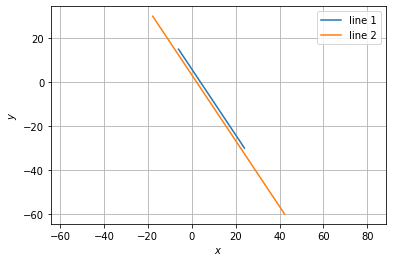
\includegraphics[width= \columnwidth]{solutions/sep/2/5/b/download4.png}
\caption{Graphical solution}
\label{sep/2/5/b/Fig:Graphical Solution}
\end{figure}
